\section{Static Convex Hull Construction\label{sec:convex_hull_3}}

\ccIndexSubitem{convex hull, 3D}{static}
\ccIndexSubitem{convex hull, 3D}{quickhull}

The function 
\ccc{convex_hull_3}\ccIndexMainItem[C]{convex_hull_3} provides an 
implementation of the quickhull algorithm \cite{bdh-qach-96} for three 
dimensions\ccIndexMainItem{quickhull, 3D}.  There are two versions of this
function available, one that can be used when it is known that the output
will be a polyhedron (\textit{i.e.}, there are more than three points and
they are not all collinear) and one that handles all degenerate cases
and returns a \ccc{CGAL::Object}, which may be a point, a segment, a
triangle, or a polyhedron.  Both versions accept a range of input
iterators defining the set of points whose convex hull is to be computed
and a traits class defining the geometric types and predicates used in
computing the hull.

\subsection{Traits Class}

The function \ccc{convex_hull_3} is parameterized by a traits class,
which specifies the types and geometric primitives to be used in the
computation. If input points from a kernel with exact predicates 
and non-exact constructions are used, and a certified result is expected,
the traits \ccc{Convex_hull_traits_3<R>} should be used 
(\ccc{R} being the input kernel). Note that the default traits class takes this into
account.

\subsection{Convexity Checking}

The function \ccc{is_strongly_convex_3}\ccIndexMainItem[C]{is_strongly_convex_3}
implements the algorithm of Mehlhorn \textit{et al.} \cite{mnssssu-cgpvg-96} 
to determine if the vertices of a given polytope constitute a strongly convex 
point set or not.  This function is used in postcondition testing for
\ccc{convex_hull_3}\ccIndexSubitem[C]{convex_hull_3}{postcondition}.

\subsection{Example}
The following program computes the convex hull of a set of 250 random
points chosen from a sphere of radius 100.  It then determines if the 
resulting hull is a segment or a polyhedron.  

\ccIncludeExampleCode{Convex_hull_3/quickhull_3.cpp}


\section{Incremental  Convex Hull Construction}
\ccIndexSubitem{convex hull, 3D}{incremental}

The function \ccc{convex_hull_incremental_3} %
\ccIndexMainItem[C]{convex_hull_incremental_3} provides an
interface similar to \ccc{convex_hull_3} for the $d$-dimensional 
incremental construction algorithm \cite{cms-frric-93}  
implemented by the class \ccc{CGAL::Convex_hull_d<R>} that is specialized 
to three dimensions. This function accepts an iterator range over a set of
input points and returns a polyhedron, but it does not have a traits class
in its interface.  It uses the kernel
class \ccc{Kernel} used in the polyhedron type to define an instance of the 
adapter traits class \ccc{CGAL::Convex_hull_d_traits_3<Kernel>}.

In almost all cases, the static and the dynamic version  will
be faster than the incremental convex hull algorithm (mainly
because of the lack of efficient filtering and the overhead
of the general d-dimension). The incremental version is provided for
completeness and educational purposes. You  should use the dynamic
version when you need an  efficient incremental  convex hull algorithm. 


To use the full functionality available with the $d$-dimensional class 
\ccc{CGAL::Convex_hull_d<R>} in three dimensions (\textit{e.g.}, the ability
to insert new points and to query if a point lies in the convex hull or not), 
you can instantiate the class \ccc{CGAL::Convex_hull_d<K>} with the adapter
traits class \ccc{CGAL::Convex_hull_d_traits_3<K>}, as shown in the following
example.

\subsection{Example}

\ccIncludeExampleCode{Convex_hull_3/incremental_hull_class_3.cpp}

\section{Dynamic  Convex Hull Construction}
\ccIndexSubitem{convex hull, 3D}{dynamic}

Fully dynamic maintenance of a convex hull can be achieved by using the
class \ccc{CGAL::Delaunay_triangulation_3}.  This class supports insertion
and removal of points (\textit{i.e.}, vertices of the triangulation) and the 
convex hull edges are simply the finite edges of infinite faces.  
The following example illustrates the dynamic construction of a convex hull.
First, random points from a sphere of a certain radius are generated and are
inserted into a triangulation.  Then the number of points of the convex hull 
are obtained by counting the number of triangulation vertices incident to the 
infinite vertex.  Some of the points are removed and then the number of points 
remaining on the hull are determined.  Notice that the vertices incident to the
infinite vertex of the triangulation are on the convex hull but it may be that
not all of them are vertices of the hull.

\subsection{Example}
\ccIncludeExampleCode{Convex_hull_3/dynamic_hull_3.cpp}

\section{Performance}

\begin{figure}
\begin{ccTexOnly}
\begin{center}
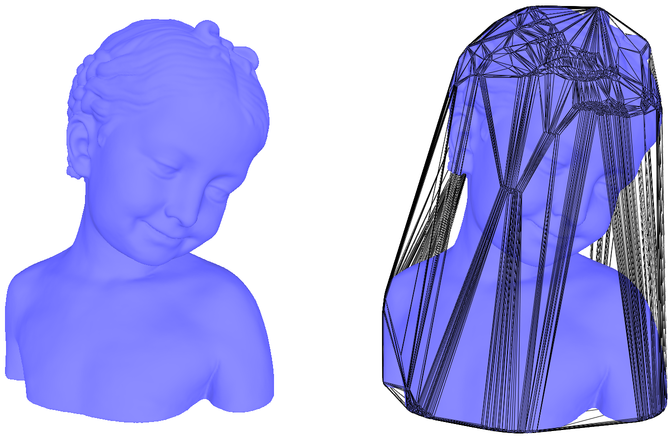
\includegraphics[width=12cm]{Convex_hull_3/chull_bimba.png}
\end{center}
\end{ccTexOnly}
\begin{ccHtmlOnly}
<CENTER>
<img border=0 src="./chull_bimba.png" alt="the convex hull of the bimba model">
</CENTER>
\end{ccHtmlOnly}
\caption{The convex hull of a model made of 192135 points.
\label{fig-ch-bimba}}
\end{figure}

In the following, we compare the running times of the three approaches to compute 3D convex hulls.
For the static version (using \ccc{CGAL::convex_hull_3}) and the dynamic version
(using \ccc{CGAL::Delaunay_triangulation_3} and \ccc{CGAL::convex_hull_3_to_polyhedron_3}), the kernel
used was \ccc{CGAL::Exact_predicates_inexact_constructions_kernel}. For the incremental version
(using \ccc{CGAL::convex_hull_incremental_3}), the kernel used was \ccc{CGAL::Exact_predicates_exact_constructions_kernel}.

To compute the convex hull of a million of random points in a unit ball the static approach needed 1.63s, while 
the dynamic and incremental approaches needed 9.50s and 11.54s respectively.
To compute the convex hull of the model of Figure \ref{fig-ch-bimba} featuring 192135 points, 
the static approach needed 0.18s, while the dynamic and incremental approaches needed 1.90s and 6.80s respectively.

The measurements have been performed using \cgal\ 3.9, using the \gnu\ \CC\  compiler version 4.3.5, under Linux (Debian distribution),
with the compilation options \texttt{-O3 -DCGAL\_NDEBUG}. The computer used was equipped with a 64bit Intel Xeon 2.27GHz processor and 12GB of RAM.